\documentclass[10pt]{article}

%This is the minimal setup required to render the flag
\usepackage[paperwidth=12cm, paperheight=8cm, top=0cm, bottom=0cm, left=0cm, right=0cm]{geometry}
%Paper width is set to 12cm by 8 cm to match the Chilean Government-specified aspect ratio (3:2)
\usepackage{tikz}
%\usepackage[dvipsnames]{xcolor} % Optional unless you want to use colors pre-defined by the xcolor package

% Colors for the flag (the Chilean government does not specify exact colors)
\definecolor{chred}{RGB}{213,43,30}
\definecolor{chwhite}{RGB}{255,255,255}
\definecolor{chblue}{RGB}{0,57,166}

% Other government specifications include:
% Canton (blue) is a square of side length 1/2 flag height, here it is 4cm
% Diameter of star is 1/4 flag width, here it is 2cm

%Sources:
%https://www.fotw.info/flags/cl.html
%https://en.wikipedia.org/wiki/Flag_of_Chile

%Created by Senan Sekhon, August 3, 2021

\begin{document}

\begin{center} %Optional, but helps to tidy up the layout
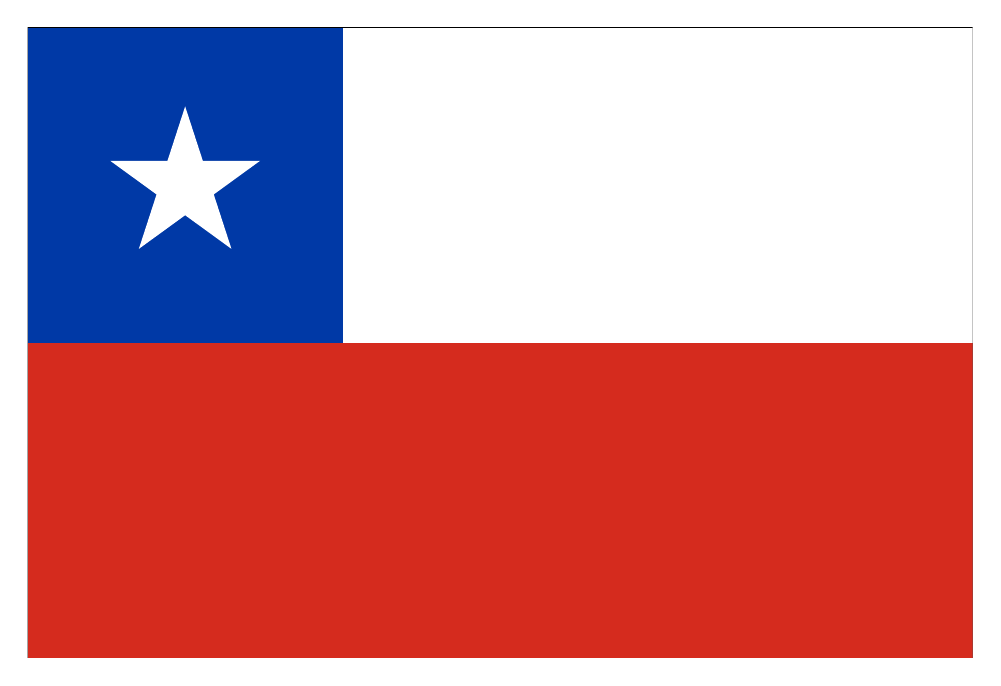
\begin{tikzpicture}[scale=1]
\clip (-6,-4) rectangle (6,4); %Optional, crops the flag to the correct size
\draw[-] (-6,-4) rectangle (6,4); %Optional, draws a border around the flag
\fill[chred] (-6,-4) rectangle (6,0); %Lower portion (red)
\fill[chwhite] (-2,0) rectangle (6,4); %Upper portion (white)
\fill[chblue] (-6,0) rectangle (-2,4); %Canton (blue)
\begin{scope}[shift={(-4,2)}] %Star
\fill[chwhite] (90:1)--(54:{(3-sqrt(5))/2})--(18:1)--(-18:{(3-sqrt(5))/2})--(-54:1)--(-90:{(3-sqrt(5))/2})--(-126:1)--(-162:{(3-sqrt(5))/2})--(-198:1)--(-234:{(3-sqrt(5))/2})--cycle;
\end{scope}
\end{tikzpicture}
\end{center}

\end{document}